\section{Resultados da modelagem na coorte aceita}
\label{sec:resultados}

\subsection{Distribuição da popularidade e presença de valores elevados}

A popularidade das 58.633 composições apresentou média de 26,01 pontos, mediana de 25 e desvio-padrão de 13,44. Metade das observações estava entre 16 e 34 pontos; o percentil 95 foi 51 e o percentil 99 foi 62. O máximo observado foi 85, e 246 composições tinham valor zero. Esses números mostram que a maior parte da coorte está concentrada nas regiões baixa e intermediária da escala, com uma cauda à direita.

\begin{table}[htbp]
\centering\small
\caption{Distribuição das composições por faixa de popularidade}\label{tab:distribuicao}
\begin{tabular}{lrr}
\toprule
Popularidade & Composições & Participação (\%)\\\midrule
0 a 9 & 5.694 & 9,711\\
10 a 19 & 14.822 & 25,279\\
20 a 29 & 16.747 & 28,562\\
30 a 39 & 12.138 & 20,702\\
40 a 49 & 5.799 & 9,890\\
50 a 59 & 2.512 & 4,284\\
60 a 69 & 772 & 1,317\\
70 a 79 & 138 & 0,235\\
80 a 89 & 11 & 0,019\\
90 a 100 & 0 & 0,000\\
Total & 58.633 & 100,000\\
\bottomrule
\end{tabular}
\fonte{Elaboração a partir dos resultados salvos da coorte aceita.}
\nota{As faixas referem-se à resposta observada; não foram usadas para excluir observações. Percentuais arredondados podem não somar exatamente 100.}
\end{table}


\textbf{As 11 observações mencionadas na análise correspondem somente às composições com popularidade entre 80 e 89 pontos.} Elas representam aproximadamente 0,019\% da amostra de desenvolvimento. Não são as únicas músicas consideradas populares em qualquer sentido: havia também 138 composições entre 70 e 79 e 772 entre 60 e 69. Ao considerar valores iguais ou superiores a 70, o total é 149; com limiar de 60, são 921. Não houve observação de 90 a 100 nessa matriz. Esses limiares são faixas descritivas, não categorias universais de sucesso.

O número pequeno não resulta de treinamento feito com apenas 11 músicas, nem de exclusão das que o modelo errou. Todas as 58.633 composições foram incluídas na avaliação OOF. A contagem de 11 decorre da distribuição da resposta na coorte resultante da integração, da disponibilidade de letras aceitas, do split preservado e da seleção de representantes. Como não houve amostragem com cotas iguais de popularidade, não se garantiu um número mínimo de casos na cauda.

Não é possível atribuir esse desequilíbrio a uma única causa com os resumos disponíveis. Há, porém, evidência descritiva de cobertura desigual: no nível de faixa do desenvolvimento, as 58.705 faixas com letras aceitas apresentaram popularidade média de 26,01, enquanto as 25.112 sem letra aceita tiveram média de 29,76. Isso indica que condicionar a análise à disponibilidade de letra modifica o perfil observado. Não demonstra que a obtenção de letra cause menor popularidade, nem que o LRCLIB seja a única origem da diferença.

Consequentemente, a amostra não deve ser descrita como retrato representativo de todas as músicas do Spotify. Ter muitas observações reduz algumas fontes de instabilidade, mas não corrige automaticamente seleção da base ou escassez em determinadas regiões da resposta. A Figura~\ref{fig:distribuicao} apresenta a distribuição empírica; o gráfico QQ marginal não constitui teste dos pressupostos dos resíduos de uma regressão.

\begin{figure}[htbp]
\centering
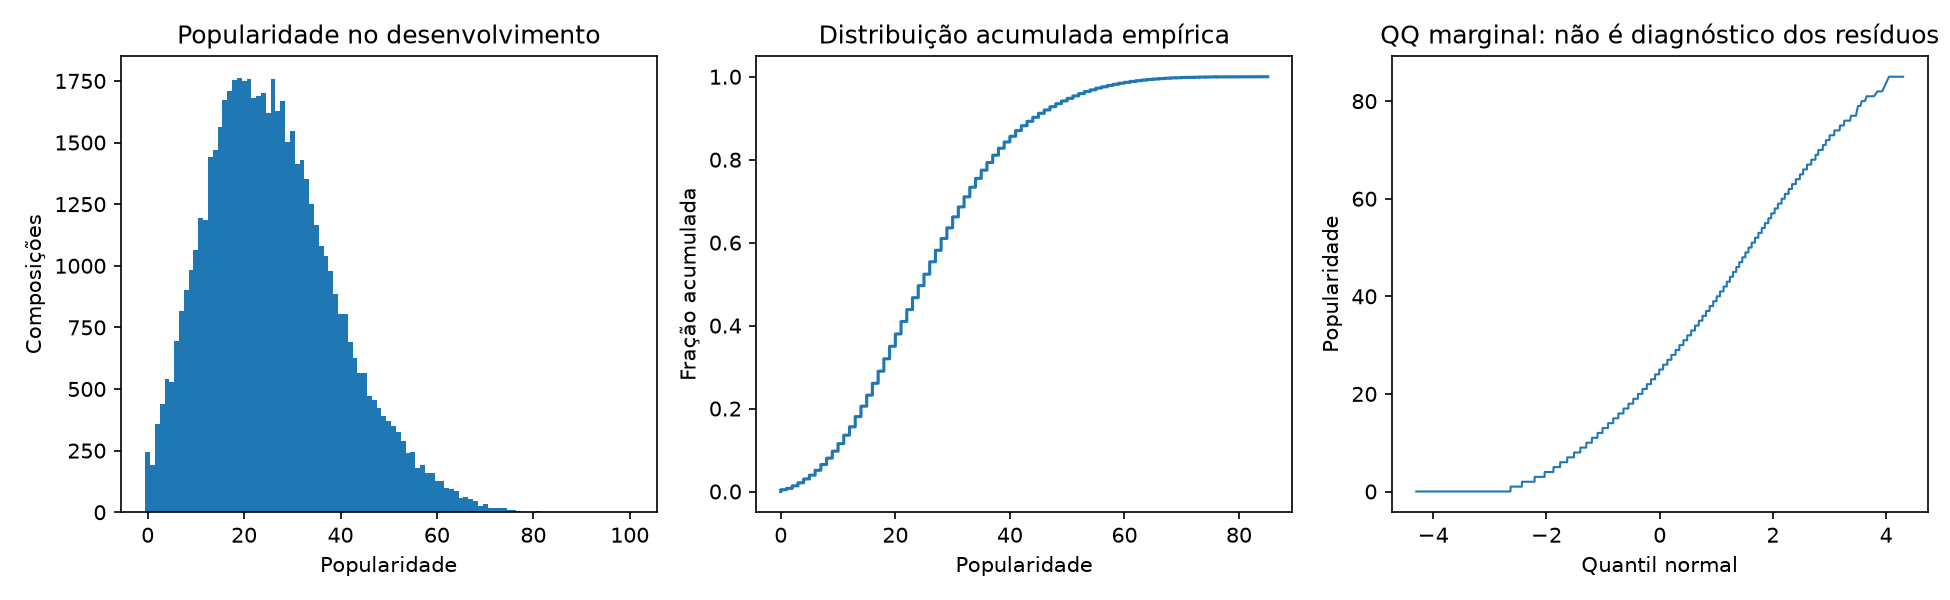
\includegraphics[width=\textwidth]{images/distribuicao_popularidade.png}
\caption{Distribuição, frequência acumulada e gráfico QQ marginal da popularidade no desenvolvimento}\label{fig:distribuicao}
\fonte{Análise descritiva da coorte aceita. Figura original preservada.}
\end{figure}

\subsection{Comparação das famílias de regressão}

A Tabela~\ref{tab:modelos} apresenta os resultados globais de validação cruzada. Todas as linhas foram avaliadas sobre as mesmas 58.633 composições, permitindo comparação direta dentro desta rodada. Não se trata de comparar erros de treinamento.

\begin{table}[htbp]
\centering\small
\caption{Desempenho OOF das famílias de regressão}\label{tab:modelos}
\begin{tabular}{llrrr}
\toprule
Família & Bloco & MAE & RMSE & $R^2$\\\midrule
Linear comum & Baseline & 7,0536 & 9,1360 & 0,5378\\
Linear comum & Tradicional & 6,9854 & 9,0549 & 0,5460\\
Ridge & Baseline & 7,0524 & 9,1340 & 0,5380\\
Ridge & Tradicional & 6,9712 & 9,0269 & 0,5488\\
Elastic Net & Baseline & 7,4490 & 9,6340 & 0,4860\\
Elastic Net & Tradicional & 7,3577 & 9,5095 & 0,4992\\
Aditiva Ridge & Baseline & 6,9546 & 8,9924 & 0,5522\\
Aditiva Ridge & Tradicional & 6,8906 & 8,9016 & 0,5612\\
Média do treino & Constante & 10,7488 & 13,4383 & $\approx 0$\\
Mediana do treino & Constante & 10,7003 & 13,4760 & -0,0056\\
\bottomrule
\end{tabular}
\fonte{Elaboração a partir dos resultados salvos da coorte aceita.}
\nota{n = 58.633 para todas as linhas. Valores menores favorecem MAE/RMSE; maiores favorecem R². A escolha interna de família também selecionou a aditiva nos cinco folds de cada bloco.}
\end{table}


A regressão aditiva com Ridge apresentou os menores MAE e RMSE e o maior $R^2$ entre as famílias examinadas, nos dois blocos. Além disso, ela foi escolhida pela validação interna nos cinco folds de cada bloco. Portanto, a preferência por essa família não decorreu apenas de olhar retrospectivamente a tabela externa: o procedimento de seleção interno também a indicou em todas as rodadas.

As referências constantes ajudam a interpretar a magnitude do desempenho. A previsão pela mediana do treino apresentou MAE de 10,7003, enquanto o Tradicional aditivo atingiu 6,8906. A redução relativa foi de aproximadamente 35,6\%. Isso mostra informação preditiva em relação a prever a mesma popularidade para todas as músicas. Não significa que o modelo explique toda a popularidade ou seja suficientemente preciso para qualquer aplicação individual.

No Baseline, a passagem da regressão linear comum para a aditiva reduziu o MAE de 7,0536 para 6,9546. Esse contraste sugere que permitir relações curvas trouxe benefício preditivo nesta amostra, sem provar um mecanismo causal. Separadamente, a comparação entre Baseline aditivo e Tradicional aditivo avalia o acréscimo do bloco textual sob a mesma família de modelos.

O Elastic Net foi menos competitivo dentro da grade definida nesta rodada. Isso não permite concluir que o método seja inadequado em geral: as penalizações aqui avaliadas foram limitadas e diferem das utilizadas em etapas anteriores. Não foram realizados novos ajustes após observar os resultados para tentar melhorar sua posição na comparação.

\subsection{Quanto os descritores de letras acrescentaram}

\begin{table}[htbp]
\centering\small
\caption{Contribuição dos descritores na regressão aditiva com Ridge}\label{tab:incremento}
\begin{tabular}{lrrr}
\toprule
Métrica & Baseline & Tradicional & Diferença T--B\\\midrule
MAE & 6,9546 & 6,8906 & -0,0639\\
RMSE & 8,9924 & 8,9016 & -0,0908\\
$R^2$ & 0,5522 & 0,5612 & 0,0090\\
P95 do erro absoluto & 17,6078 & 17,4403 & -0,1675\\
Erros acima de 20 & 1.945 & 1.882 & -63\\
\bottomrule
\end{tabular}
\fonte{Elaboração a partir dos resultados salvos da coorte aceita.}
\nota{Diferenças negativas são favoráveis para medidas de erro. Para R², diferenças positivas são favoráveis.}
\end{table}


O Tradicional aditivo reduziu o MAE em 0,06395 ponto, aproximadamente 0,92\%, em relação ao Baseline aditivo. O RMSE diminuiu 0,09082 ponto e o $R^2$ aumentou aproximadamente 0,009. Houve melhora simultânea do MAE, do RMSE e do P95, acompanhada de redução de 1.945 para 1.882 erros acima de 20 pontos.

Esses 63 erros grandes a menos correspondem a uma redução relativa de aproximadamente 3,24\% nessa contagem. Na proporção sobre toda a amostra, a frequência passou de aproximadamente 3,32\% para 3,21\%, diferença de cerca de 0,11 ponto percentual. É importante distinguir essas duas medidas: redução relativa na contagem de erros não é a mesma coisa que redução em pontos percentuais.

O intervalo exploratório de 95\% para a diferença de MAE, Tradicional menos Baseline, foi de $-0,08395$ a $-0,04501$ ponto. Para a diferença de RMSE, o intervalo foi de $-0,11348$ a $-0,06941$. Os intervalos ficaram abaixo de zero, compatíveis com um ganho consistente sob a reamostragem utilizada. Entretanto, a magnitude do ganho continuou pequena: uma evidência estatística de diferença não implica uma melhora prática expressiva.

A interpretação adequada é que os descritores disponíveis acrescentaram informação preditiva às características do Baseline, mas não alteraram de forma radical a precisão das estimativas. Esse resultado é relevante para a pergunta do estudo: ele quantifica o benefício incremental, inclusive quando esse benefício é modesto. Não há necessidade de obter um ganho grande para que a comparação seja cientificamente informativa.

\subsection{Estabilidade entre as partes de validação}

\begin{table}[htbp]
\centering\small
\caption{MAE e erros grandes por fold nos modelos aditivos}\label{tab:estabilidade}
\begin{tabular}{crrrrr}
\toprule
Fold & MAE B & MAE T & $\Delta$MAE & Erros >20 B & Erros >20 T\\\midrule
1 & 6,9317 & 6,8370 & -0,0947 & 389 & 364\\
2 & 7,1595 & 7,0598 & -0,0997 & 417 & 396\\
3 & 6,9849 & 6,9208 & -0,0640 & 405 & 382\\
4 & 6,9283 & 6,8910 & -0,0374 & 387 & 386\\
5 & 6,7629 & 6,7400 & -0,0228 & 347 & 354\\
\bottomrule
\end{tabular}
\fonte{Elaboração a partir dos resultados salvos da coorte aceita.}
\nota{B = Baseline; T = Tradicional. Os folds não são experimentos independentes.}
\end{table}


O Tradicional aditivo apresentou MAE, RMSE e P95 inferiores aos do Baseline aditivo nos cinco folds. Essa repetição da direção do resultado reduz a impressão de que o ganho agregado tenha surgido em uma única partição favorável. As magnitudes, porém, variaram: a redução do MAE foi menor no quinto fold do que nos dois primeiros.

A redução de erros acima de 20 pontos não foi uniforme. O Tradicional teve menos erros grandes em quatro folds, mas no quinto a contagem aumentou de 347 para 354. Assim, a afirmação de estabilidade deve ser específica: as três métricas MAE, RMSE e P95 melhoraram em todos os folds, enquanto a frequência de erros grandes melhorou em quatro dos cinco.

A penalização Ridge escolhida foi igual a 1 em todos os folds dos modelos aditivos. No Tradicional, a transformação \texttt{asinh} dos descritores foi selecionada em quatro folds; no quinto, foram escolhidos os valores originais. Esses parâmetros foram selecionados no treinamento interno, sem consulta ao desempenho externo para decidir qual configuração usar.

\subsection{Em quais músicas o modelo teve maior dificuldade}

\begin{table}[htbp]
\centering\small
\caption{Erros dos modelos aditivos por faixa da resposta}\label{tab:erros_faixas}
\begin{tabular}{lrrrr}
\toprule
Popularidade & n & MAE B & MAE T & Erros >20 T (\%)\\\midrule
0 a 9 & 5.694 & 8,81 & 8,65 & 3,04\\
10 a 19 & 14.822 & 6,38 & 6,28 & 0,20\\
20 a 29 & 16.747 & 5,19 & 5,19 & 0,19\\
30 a 39 & 12.138 & 5,89 & 5,91 & 1,43\\
40 a 49 & 5.799 & 8,70 & 8,61 & 7,59\\
50 a 59 & 2.512 & 13,95 & 13,64 & 22,21\\
60 a 69 & 772 & 19,76 & 19,30 & 48,58\\
70 a 79 & 138 & 26,30 & 25,94 & 67,39\\
80 a 89 & 11 & 33,23 & 31,98 & 81,82\\
90 a 100 & 0 & -- & -- & --\\
\bottomrule
\end{tabular}
\fonte{Elaboração a partir dos resultados salvos da coorte aceita.}
\nota{A faixa 80--89 tem apenas 11 observações; a faixa 90--100 está vazia. Não se calculou R² dentro das faixas.}
\end{table}


O desempenho não foi homogêneo ao longo da popularidade. No Tradicional aditivo, o MAE foi de 5,19 pontos na faixa de 20 a 29, subindo para 19,30 entre 60 e 69, 25,94 entre 70 e 79 e 31,98 entre 80 e 89. Portanto, o MAE global de 6,89 não deve ser interpretado como precisão típica para uma música de popularidade muito elevada.

O erro global é uma média ponderada pelo número de observações: regiões com milhares de composições têm maior peso que a faixa com apenas 11. O bom desempenho na região central pode coexistir com erros grandes na cauda. As poucas observações extremas também limitam a precisão de qualquer conclusão específica sobre essa faixa. Não se deve generalizar o MAE calculado para as 11 composições como se fosse uma estimativa precisa para todos os grandes sucessos.

Há ainda compromissos locais: nas faixas de 20 a 29 e de 30 a 39, o MAE do Tradicional foi ligeiramente maior que o do Baseline, embora o resultado global tenha melhorado. Acrescentar descritores não garantiu melhora em toda faixa ou em toda música. A comparação por subgrupos complementa, portanto, a tabela global.

\subsection{Resíduos e limites da representação ajustada}

Define-se o resíduo como popularidade observada menos prevista. Resíduos positivos indicam subestimação; negativos indicam superestimação. O gráfico QQ dos resíduos OOF apresenta afastamento da referência normal, especialmente na cauda superior. Há erros positivos e negativos de grande magnitude. A inspeção visual não sustenta assumir erros perfeitamente normais ou construir intervalos individuais apenas somando e subtraindo o MAE.

O painel de resíduos versus previsões e o de escala-localização também mostram que a dispersão deve ser examinada ao longo dos valores previstos. Esses gráficos fornecem indícios descritivos, não um teste formal de homocedasticidade. O desempenho por faixas da resposta evidencia diretamente que a dificuldade preditiva varia entre regiões da escala.

O Baseline aditivo produziu 72 previsões negativas, e o Tradicional aditivo produziu 60; nenhum dos dois gerou previsão acima de 100. Como essas regressões não impõem automaticamente os limites da resposta, os valores negativos são possíveis. Eles foram mantidos para que a avaliação refletisse o procedimento realmente ajustado, sem correção posterior que modificasse as métricas. A Figura~\ref{fig:residuos} reúne os diagnósticos do Tradicional aditivo.

\FloatBarrier
\begin{landscape}
\begin{figure}[p]
\centering
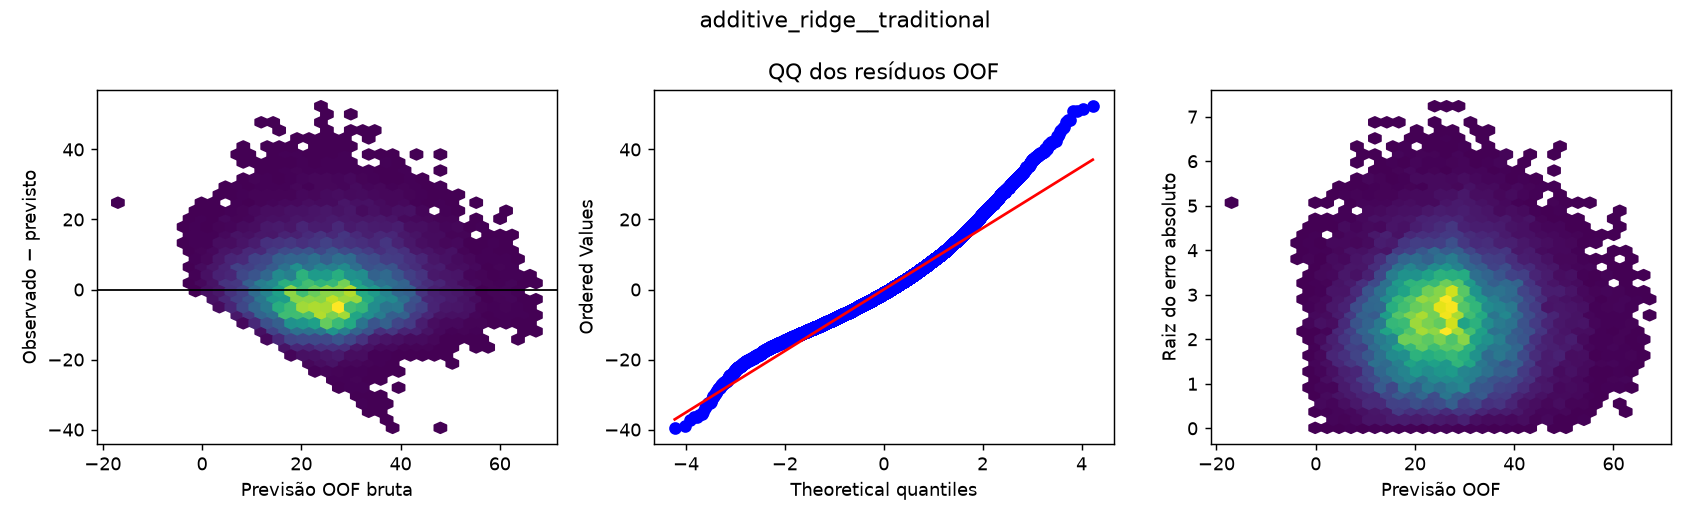
\includegraphics[width=\linewidth]{images/residuos_tradicional_aditivo.png}
\caption{Diagnósticos dos resíduos OOF da regressão aditiva com Ridge no bloco Tradicional}\label{fig:residuos}
\fonte{Execução da modelagem da coorte aceita. Figura original preservada.}
\nota{À esquerda, resíduos versus previsões; ao centro, gráfico QQ; à direita, raiz do erro absoluto versus previsões. A orientação horizontal permite ler os três painéis. Nenhuma previsão foi recalibrada para produzir esta figura.}
\end{figure}
\end{landscape}
